\pdfinfoomitdate=1
\pdftrailerid{}
\pdfsuppressptexinfo=-1
\documentclass[10pt,a4paper]{article}
\usepackage{cmap}
\usepackage[margin=1.8cm,headheight=14pt,headsep=10pt]{geometry}
\usepackage[leqno]{amsmath}
\usepackage{amssymb,booktabs,longtable,array,ragged2e,multicol,multirow,xcolor,fancyhdr,tikz}
\definecolor{linkblue}{rgb}{0.08,0.33,0.58}
\usepackage[colorlinks=true,linkcolor=linkblue,urlcolor=linkblue,citecolor=linkblue,
  filecolor=linkblue,linktoc=all,pdfborder={0 0 0},bookmarksnumbered=true]{hyperref}
\setlength{\parindent}{0pt}\setlength{\parskip}{4pt}
\setcounter{secnumdepth}{2}\setcounter{tocdepth}{2}
\definecolor{partshade}{gray}{0.9}
\definecolor{parttitle}{HTML}{7A1466}
\definecolor{parttitlelight}{HTML}{D66EBC}
\makeatletter
\renewcommand\section{\@startsection{section}{1}{\z@}{-3ex plus -1ex minus -.2ex}%
  {1.2ex plus .2ex}{\normalfont\large\sffamily\bfseries\color{parttitle}}}
\renewcommand\subsection{\@startsection{subsection}{2}{\z@}{-2.5ex plus -1ex minus -.2ex}%
  {.8ex plus .2ex}{\normalfont\sffamily\bfseries\color{parttitle}}}
\renewcommand\subsubsection{\@startsection{subsubsection}{3}{\z@}{-2ex plus -1ex minus -.2ex}%
  {.6ex plus .2ex}{\normalfont\small\sffamily\bfseries\color{parttitle}}}
\renewcommand\paragraph{\@startsection{paragraph}{4}{\z@}{1.5ex plus .5ex minus .2ex}{-1em}%
  {\normalfont\small\sffamily\bfseries\color{parttitle}}}
\renewcommand\tagform@[1]{\maketag@@@{\textsf{\bfseries\footnotesize (#1)}}}
\renewcommand*\l@part[2]{\par\addvspace{1.6ex}\noindent{\sffamily\bfseries #1}\hfill
  {\sffamily\bfseries #2}\par\nobreak}
\newcommand\tocnumber{1.8em}
\newcommand\tocline[4]{\par{\rightskip \tocnumber plus 1fil\relax\parfillskip -\rightskip
  \noindent\hangindent\dimexpr#1+#2\relax\hspace*{#1}%
  \@tempdima #2{\sffamily\small #3}\nobreak\leaders\hbox{$\m@th\mkern 4.5mu\hbox{.}%
  \mkern 4.5mu$}\hfill\nobreak\hbox to \tocnumber{\hfil\sffamily\small #4}\par}}
\renewcommand*\l@section[2]{\tocline{0em}{2.2em}{#1}{#2}}
\renewcommand*\l@subsection[2]{\tocline{2.2em}{2.6em}{#1}{#2}}
\newcommand\contentspage{{\setlength{\columnsep}{24pt}\begin{multicols}{2}\@starttoc{toc}%
  \end{multicols}}}
\newcounter{docpart}\@addtoreset{section}{docpart}
\renewcommand\thesection{\ifnum\value{docpart}>0 \arabic{docpart}.\fi\arabic{section}}
\renewcommand\theHsection{\arabic{docpart}.\arabic{section}}
\newcommand\partnumber[1]{#1\enspace}
\pdfstringdefDisableCommands{\def\partnumber#1{#1 }}
\newcommand{\partbox}[1]{\par\addvspace{12pt}\refstepcounter{docpart}\phantomsection
  \addcontentsline{toc}{part}{\protect\partnumber{\thedocpart}#1}%
  \noindent\colorbox{partshade}{\makebox[%
  \dimexpr\textwidth-2\fboxsep\relax]{\rule[-6pt]{0pt}{20pt}\Large\sffamily\bfseries%
  \textcolor{parttitle}{\thedocpart\quad #1}}}\par\nobreak\@nobreaktrue\addvspace{2pt}}
\newmarks\LTstartmarks\newcount\LTstartcount
\let\LT@startplain\LT@start
\def\LT@start{\global\advance\LTstartcount\@ne\LT@startplain
  \marks\LTstartmarks{\the\LTstartcount}}
\newmarks\LTgroupmarks
\newcount\LTspacebreak\LTspacebreak=-1
\newcount\LTrulebreak\LTrulebreak=-2
\def\grouprule#1#2{\noalign{\marks\LTgroupmarks{\the\belowrulesep}\nobreak\vskip#1%
  \vskip\aboverulesep}\multispan\LT@cols\unskip{\leaders\hrule\@height#2\hfill\kern\z@}\cr
  \noalign{\penalty\LTrulebreak\vskip\belowrulesep\global\@lastruleclass\z@}}
\def\groupspace#1{\noalign{\marks\LTgroupmarks{\the\dimexpr#1\relax}\penalty\LTspacebreak
  \vskip#1\global\@lastruleclass\z@}}
\def\LT@unskips{\unskip\unpenalty\unskip\unpenalty\unskip\unpenalty\unskip\unpenalty}
\def\LT@groupcut{\ifnum\outputpenalty=\LTrulebreak
  \setbox\@cclv\vbox{\unvbox\@cclv\setbox\z@\lastbox\LT@unskips}\fi}
\def\LT@groupjoin{\ifnum\outputpenalty=\LTspacebreak\vskip-\botmarks\LTgroupmarks\relax\fi
  \ifnum\outputpenalty=\LTrulebreak\vskip-\botmarks\LTgroupmarks\relax\fi}
\let\LT@outputplain\LT@output
\def\LT@output{\ifnum\outputpenalty<-\@Mi\LT@outputplain\else
  \edef\LT@marka{\botmarks\LTstartmarks}\edef\LT@markb{\the\LTstartcount}%
  \ifx\LT@marka\LT@markb\LT@groupcut\LT@outputplain\LT@groupjoin
  \else\setbox\LT@head\box\voidb@x\LT@outputplain\fi\fi}
\makeatother
\newcommand{\needspace}[1]{\par\penalty-100\begingroup\dimen0=#1\relax\dimen2=\pagegoal
  \advance\dimen2-\pagetotal\ifdim\dimen0>\dimen2\relax\ifdim\dimen2>0pt\vfil\break\fi\fi
  \endgroup}
\numberwithin{equation}{section}
\pagestyle{fancy}\fancyhf{}
\renewcommand{\headrulewidth}{0pt}
\renewcommand{\sectionmark}[1]{\markright{\thesection\enspace #1}}
\renewcommand{\subsectionmark}[1]{}
\fancyhead[R]{\small\textsc{\rightmark}\quad\thepage}
\fancypagestyle{plain}{\fancyhf{}\fancyfoot[C]{\small\thepage}}
\definecolor{atlasI}{HTML}{991A1A}\definecolor{atlasIl}{HTML}{EC6B60}
\definecolor{atlasII}{HTML}{295A2C}\definecolor{atlasIIl}{HTML}{6C9F6D}
\definecolor{atlasIII}{HTML}{7A1466}\definecolor{atlasIIIl}{HTML}{D66EBC}
\definecolor{atlasIV}{HTML}{9B690B}\definecolor{atlasIVl}{HTML}{F2A618}
\makeatletter
\newcommand\atlas@full{%
\fill[atlasIII] (0.0394,0.0163) -- (0.3978,0.0163) arc[start angle=0.668, end angle=13.836, radius=1.3979] -- cycle;
\fill[atlasI] (-0.0163,0.0394) -- (-0.0163,0.3978) arc[start angle=90.668, end angle=103.836, radius=1.3979] -- cycle;
\fill[atlasIV] (-0.0394,-0.0163) -- (-0.3978,-0.0163) arc[start angle=-179.332, end angle=-166.164, radius=1.3979] -- cycle;
\fill[atlasII] (0.0163,-0.0394) -- (0.0163,-0.3978) arc[start angle=-89.332, end angle=-76.164, radius=1.3979] -- cycle;
\fill[atlasIIIl] (0.0163,0.0394) -- (0.3343,0.3573) arc[start angle=76.164, end angle=89.332, radius=1.3979] -- cycle;
\fill[atlasIl] (-0.0394,0.0163) -- (-0.3573,0.3343) arc[start angle=166.164, end angle=179.332, radius=1.3979] -- cycle;
\fill[atlasIVl] (-0.0163,-0.0394) -- (-0.3343,-0.3573) arc[start angle=-103.836, end angle=-90.668, radius=1.3979] -- cycle;
\fill[atlasIIl] (0.0394,-0.0163) -- (0.3573,-0.3343) arc[start angle=-13.836, end angle=-0.668, radius=1.3979] -- cycle;
\fill[atlasIIIl] (0.4304,0.0163) -- (0.9598,0.0163) arc[start angle=46.637, end angle=73.849, radius=1.3979] arc[start angle=13.862, end angle=0.653, radius=1.4305] -- cycle;
\fill[atlasIl] (-0.0163,0.4304) -- (-0.0163,0.9598) arc[start angle=136.637, end angle=163.849, radius=1.3979] arc[start angle=103.862, end angle=90.653, radius=1.4305] -- cycle;
\fill[atlasIVl] (-0.4304,-0.0163) -- (-0.9598,-0.0163) arc[start angle=-133.363, end angle=-106.151, radius=1.3979] arc[start angle=-166.138, end angle=-179.347, radius=1.4305] -- cycle;
\fill[atlasIIl] (0.0163,-0.4304) -- (0.0163,-0.9598) arc[start angle=-43.363, end angle=-16.151, radius=1.3979] arc[start angle=-76.138, end angle=-89.347, radius=1.4305] -- cycle;
\fill[atlasIII] (0.0163,0.4304) arc[start angle=89.347, end angle=76.138, radius=1.4305] arc[start angle=16.151, end angle=43.363, radius=1.3979] -- cycle;
\fill[atlasI] (-0.4304,0.0163) arc[start angle=179.347, end angle=166.138, radius=1.4305] arc[start angle=106.151, end angle=133.363, radius=1.3979] -- cycle;
\fill[atlasIV] (-0.0163,-0.4304) arc[start angle=-90.653, end angle=-103.862, radius=1.4305] arc[start angle=-163.849, end angle=-136.637, radius=1.3979] -- cycle;
\fill[atlasII] (0.4304,-0.0163) arc[start angle=-0.653, end angle=-13.862, radius=1.4305] arc[start angle=-73.849, end angle=-46.637, radius=1.3979] -- cycle;
\fill[atlasIII] (0.9997,0.0232) arc[start angle=1.329, end angle=44.066, radius=1] -- (0.3973,0.3742) arc[start angle=73.875, end angle=45.664, radius=1.4305] -- cycle;
\fill[atlasI] (-0.0232,0.9997) arc[start angle=91.329, end angle=134.066, radius=1] -- (-0.3742,0.3973) arc[start angle=163.875, end angle=135.664, radius=1.4305] -- cycle;
\fill[atlasIV] (-0.9997,-0.0232) arc[start angle=-178.671, end angle=-135.934, radius=1] -- (-0.3973,-0.3742) arc[start angle=-106.125, end angle=-134.336, radius=1.4305] -- cycle;
\fill[atlasII] (0.0232,-0.9997) arc[start angle=-88.671, end angle=-45.934, radius=1] -- (0.3742,-0.3973) arc[start angle=-16.125, end angle=-44.336, radius=1.4305] -- cycle;
\fill[atlasIIIl] (0.0232,0.9997) arc[start angle=44.336, end angle=16.125, radius=1.4305] -- (0.6955,0.7185) arc[start angle=45.934, end angle=88.671, radius=1] -- cycle;
\fill[atlasIl] (-0.9997,0.0232) arc[start angle=134.336, end angle=106.125, radius=1.4305] -- (-0.7185,0.6955) arc[start angle=135.934, end angle=178.671, radius=1] -- cycle;
\fill[atlasIVl] (-0.0232,-0.9997) arc[start angle=-135.664, end angle=-163.875, radius=1.4305] -- (-0.6955,-0.7185) arc[start angle=-134.066, end angle=-91.329, radius=1] -- cycle;
\fill[atlasIIl] (0.9997,-0.0232) arc[start angle=-45.664, end angle=-73.875, radius=1.4305] -- (0.7185,-0.6955) arc[start angle=-44.066, end angle=-1.329, radius=1] -- cycle;
}
\newcommand\atlas@draw[2]{\begin{tikzpicture}[x=\dimexpr(#1)/2\relax,y=\dimexpr(#1)/2\relax]
\useasboundingbox (-1,-1) rectangle (1,1);#2\end{tikzpicture}}
\newcommand\atlas@volume[1]{{%
\colorlet{atlasI}{parttitle}\colorlet{atlasIl}{parttitlelight}%
\colorlet{atlasII}{parttitle}\colorlet{atlasIIl}{parttitlelight}%
\colorlet{atlasIII}{parttitle}\colorlet{atlasIIIl}{parttitlelight}%
\colorlet{atlasIV}{parttitle}\colorlet{atlasIVl}{parttitlelight}%
#1}}
\newcommand\atlasmark[1]{\atlas@draw{#1}{\atlas@full}}
\newcommand\volumemark[1]{\atlas@volume{\atlasmark{#1}}}
\makeatother
\fancypagestyle{opening}{\fancyhf{}\fancyfoot[C]{\small\thepage}%
  \fancyhead[L]{\smash{\raisebox{-9.5mm}{\volumemark{12mm}}}}}
\hypersetup{pdftitle={O3-SO3: Point Group Atlas, volume III: magnetic point groups}, pdfsubject={Point Group Atlas magnetic record O3-SO3, schema point-group-atlas/magnetic/group-continuous/1}}
\fancyhead[L]{\small $\grp{O(3)}(\grp{SO(3)})$}
\DeclareMathAlphabet{\mathelt}{OT1}{cmss}{m}{sl}
\DeclareSymbolFont{eltgreek}{OML}{cmssm}{m}{it}
\DeclareMathSymbol{\eltsigma}{\mathord}{eltgreek}{"1B}
\DeclareSymbolFont{eltletters}{OT1}{cmss}{m}{sl}
\DeclareMathSymbol{g}{\mathalpha}{eltletters}{`g}
\DeclareMathSymbol{h}{\mathalpha}{eltletters}{`h}
\DeclareMathSymbol{Q}{\mathalpha}{eltletters}{`Q}
\DeclareMathSymbol{R}{\mathalpha}{eltletters}{`R}
\DeclareMathSymbol{\xi}{\mathord}{eltgreek}{"18}
\newcommand{\eltfont}[1]{{\let\sigma\eltsigma\mathelt{#1}}}
\newcommand{\grp}[1]{\mathsf{#1}}
\newcommand{\irr}[1]{\text{\normalfont\scshape #1}}
\newcommand{\conjpair}[1]{{}^{#1}}
\newcommand{\cls}[1]{\eltfont{#1}}
\newcommand{\comp}[1]{\eltfont{#1}}
\newcommand{\elt}[1]{\eltfont{#1}}
\newcommand{\hmname}[1]{#1}
\newcommand{\orbname}[1]{#1}
\newcommand{\ptag}[1]{\mathrm{#1}}
\newcommand{\dirprod}{\times}
\newcommand{\nconj}[1]{{\scriptsize$\times#1$}}
\newcommand{\clsletter}[1]{\,{\scriptsize\color{black!55}#1}}
\newcommand{\Cyc}[1]{\grp{Z_{#1}}}
\newcommand{\Dih}[1]{\grp{Dih_{#1}}}
\newcommand{\Alt}[1]{\grp{Alt_{#1}}}
\newcommand{\Sym}[1]{\grp{Sym_{#1}}}
\newcommand{\restr}[2]{#1\!\downarrow#2}
\newcommand{\vv}{\mathbf{v}}
\newcommand{\iunit}{\mathrm{i}}
\newcommand{\expe}{\mathrm{e}}
\newcommand{\goldenratio}{\varphi}
\newcommand{\rootunity}[1]{\zeta_{#1}}
\newcommand{\irrJ}[1]{D^{(#1)}}
\newcommand{\irrJp}[2]{D^{(#1,#2)}}
\newcommand{\repD}[1]{D^{#1}}
\newcommand{\irchar}[1]{\chi_{#1}}
\newcommand{\fsind}{\nu_{\mathrm{FS}}}
\newcommand{\irrprod}{\otimes}
\newcommand{\mult}{\kappa}
\newcommand{\intx}{\mu}
\newcommand{\cgnorm}{\mathcal{N}}
\newcommand{\jm}[2]{\bigl\lvert{}^{#1}_{\,#2}\bigr\rangle}
\newcommand{\prodket}[2]{\lvert {#1}\,{#2}\rangle}
\newcommand{\jahn}[1]{\mathrm{#1}}
\newcommand{\fcell}{\mathcal{D}}
\newcommand{\sympow}[2]{[#1^{#2}]}
\newcommand{\altpow}[2]{\{#1^{#2}\}}
\newcommand{\hairsp}{\mkern1mu}
\newenvironment{romanlist}{\begin{enumerate}%
\renewcommand{\labelenumi}{(\roman{enumi})}}%
  {\end{enumerate}}
\makeatletter
\newenvironment{irmatrix}[1]{\null\,\vcenter\bgroup\Let@\restore@math@cr\default@tag
  \baselineskip8\ex@ \lineskip3\ex@ \lineskiplimit\lineskip
  \ialign\bgroup\hfil$\m@th\scriptstyle##$\hfil&&\hskip#1\hfil$\m@th\scriptstyle##$\hfil\crcr}%
  {\crcr\egroup\egroup\,}
\makeatother
\newlength{\fillwidth}\newlength{\cellwidth}\newlength{\colwidth}
\newcommand{\cellmax}[1]{\settowidth{\cellwidth}{#1}%
  \ifdim\cellwidth>\colwidth\setlength{\colwidth}{\cellwidth}\fi}
\newcommand{\fillcap}{\ifdim\colwidth<\fillwidth\setlength{\fillwidth}{\colwidth}\fi}
\newcommand{\signbreak}{\penalty100\relax}
\begin{document}
\thispagestyle{opening}
\begin{center}
{\LARGE\sffamily\bfseries\color{parttitle}The $\grp{O(3)}(\grp{SO(3)})$ subgroup of $\grp{O(3)1'}$}
\end{center}
\contentspage
\needspace{194pt}
\partbox{The group}
\section{Names and structure}\label{s:identification}
Conventions: \href{../../CONVENTIONS.pdf}{CONVENTIONS.pdf}, sections \href{../../../rotation/CONVENTIONS.pdf\#conv.0.1}{0.1}, \href{../../../rotation/CONVENTIONS.pdf\#conv.2}{2}, \href{../../../rotation/CONVENTIONS.pdf\#conv.3}{3}, \href{../../../rotation/CONVENTIONS.pdf\#conv.11}{11}, \href{../../../rotation/CONVENTIONS.pdf\#conv.16}{16}, \href{../../CONVENTIONS.pdf\#conv.30}{30}, \href{../../CONVENTIONS.pdf\#conv.31.2}{31.2} and \href{../../CONVENTIONS.pdf\#conv.37.1}{37.1}.
{\small\begin{longtable}{@{}ll@{}}\toprule
\texttt{symbol} & $\grp{O(3)}(\grp{SO(3)})$\\
\texttt{magnetic\symbol{95}type} & III\\
\texttt{G} & \href{../../../rotation/data/pdf/O3.pdf}{$\grp{O(3)}$}\\
\texttt{H} & \href{../../../rotation/data/pdf/SO3.pdf}{$\grp{SO(3)}$}, index 2\\
\texttt{antiunitary\symbol{95}character} & $\irrJp{0}{-}$\\
\grouprule{0pt}{\lightrulewidth}
\texttt{abstract\symbol{95}type} & $\grp{SO(3)}\dirprod\Cyc{2}$\\
\grouprule{0pt}{\lightrulewidth}
\texttt{images.polar\symbol{95}even} & \href{../../../rotation/data/pdf/O3.pdf}{$\grp{O(3)}$}\\
\texttt{images.axial\symbol{95}even} & \href{../../../rotation/data/pdf/SO3.pdf}{$\grp{SO(3)}$}\\
\texttt{images.polar\symbol{95}odd} & \href{../../../rotation/data/pdf/SO3.pdf}{$\grp{SO(3)}$}\\
\texttt{images.axial\symbol{95}odd} & \href{../../../rotation/data/pdf/O3.pdf}{$\grp{O(3)}$}\\
\grouprule{0pt}{\lightrulewidth}
\texttt{normalizer} & \href{O3-1p.pdf}{$\grp{O(3)1'}$}, index 2\\
\texttt{centralizer} & \href{S2-1p.pdf}{$\grp{C_{i}1'}$}\\
\grouprule{0pt}{\lightrulewidth}
\texttt{hermann\symbol{95}mauguin} & $\hmname{\infty \infty m'}$\\
\texttt{orbit\symbol{95}space} & point of \href{../../../rotation/data/pdf/O3.pdf}{$\grp{O(3)}$}, point of \href{../../../rotation/data/pdf/SO3.pdf}{$\grp{SO(3)}$}\\
\bottomrule\end{longtable}}
The field \texttt{magnetic\symbol{95}type} is III, so $\grp{O(3)}(\grp{SO(3)})$ contains the elements of $\grp{SO(3)}$ and the products of time reversal $\varTheta$ with the other elements of $\grp{O(3)}$. The fields \texttt{G} and \texttt{H} name these groups by their records (\href{../../CONVENTIONS.pdf}{CONVENTIONS.pdf}, section \href{../../CONVENTIONS.pdf\#conv.30.3}{30.3}), and \texttt{antiunitary\symbol{95}character} names the irrep $\chi$ of $\grp{O(3)}$ with kernel $\grp{SO(3)}$. The four fields \texttt{images} name the groups by which the elements move a polar or an axial vector, even or odd under time reversal (\href{../../CONVENTIONS.pdf}{CONVENTIONS.pdf}, section \href{../../CONVENTIONS.pdf\#conv.31.2}{31.2}). Each names the record of its $\grp{O(3)}$-conjugacy class, and its frame is the identity. The fields \texttt{normalizer} and \texttt{centralizer} are taken in $\grp{O(3)1'}$, and both groups are of magnetic type II. The field \texttt{orbit\symbol{95}space} names the orbit spaces of the directions under $\grp{O(3)}$ and under $\grp{SO(3)}$, each a point.
\needspace{103pt}
\section{Class space}\label{s:class_space}
Conventions: \href{../../CONVENTIONS.pdf}{CONVENTIONS.pdf}, sections \href{../../../rotation/CONVENTIONS.pdf\#conv.4}{4}, \href{../../../rotation/CONVENTIONS.pdf\#conv.16}{16}, \href{../../CONVENTIONS.pdf\#conv.30.1}{30.1}, \href{../../CONVENTIONS.pdf\#conv.32.1}{32.1} and \href{../../CONVENTIONS.pdf\#conv.37.1}{37.1}.
\leavevmode\label{n:head.component}A row is a component of the class space of $\grp{O(3)}$, as in the section Class space of the document of \href{../../../rotation/data/pdf/O3.pdf}{$\grp{O(3)}$}. \label{n:head.element}\label{n:angle.phi}A row gives the element about $z$ at each angle and the sign $\theta = \chi(g)$ of the element of $\grp{O(3)}(\grp{SO(3)})$ over each element $g$ of the component. An element of sign $-1$ is antiunitary, the product $\varTheta g$ of time reversal and an element $g$ of $\grp{O(3)}$ outside $\grp{SO(3)}$. As $\grp{O(3)}(\grp{SO(3)})$ is isomorphic to $\grp{O(3)}$, its classes are these, and its elements multiply as those of $\grp{O(3)}$ do, with their signs multiplied. The antiunitary representative $\elt{a}$ of the corepresentations (\texttt{representative}) is $\varTheta\elt{i}$. The field \texttt{frame} is the identity, so the elements of the record of $\grp{SO(3)}$ are those of $\grp{O(3)}$ with the same matrices.
\begin{center}\begin{tabular}{@{}llr@{}}\toprule
component & element & $\theta$\\\midrule
$\comp{C(\phi)}$ & $\comp{C(\phi)}$ & $+1$\\
$\comp{i\,C(\phi)}$ & $\comp{i\,C(\phi)}$ & $-1$\\
\bottomrule\end{tabular}\end{center}
\needspace{171pt}
\partbox{Representations}
\section{Families of irreps}\label{s:families}
Conventions: \href{../../CONVENTIONS.pdf}{CONVENTIONS.pdf}, sections \href{../../../rotation/CONVENTIONS.pdf\#conv.6}{6}, \href{../../../rotation/CONVENTIONS.pdf\#conv.7}{7}, \href{../../../rotation/CONVENTIONS.pdf\#conv.11}{11}, \href{../../../rotation/CONVENTIONS.pdf\#conv.16}{16}, \href{../../CONVENTIONS.pdf\#conv.32.1}{32.1} and \href{../../CONVENTIONS.pdf\#conv.37.2}{37.2}.
\leavevmode\label{n:irrep.Delta}\label{n:head.family.irreps}A row is a family of irreps $\Lambda$ of $\grp{SO(3)}$, the subgroup of the unitary elements of $\grp{O(3)}(\grp{SO(3)})$, in the order of the section Families of irreps of the document of \href{../../../rotation/data/pdf/SO3.pdf}{$\grp{SO(3)}$}. \label{n:index.dimension}\label{n:index.frobenius}\label{n:head.index.family}A row gives its dimension $d$, its Frobenius--Schur indicator $\fsind$ and the range of the index of its irreps, as in that section. \label{n:function.character}A row also gives the character $\irchar{\Lambda}(g^2)$ for the elements $g$ of $\grp{O(3)}$ outside $\grp{SO(3)}$, on their component (section~\ref{s:class_space}). The indicator $\iota$ of $\Lambda$ under the representative $\elt{a}$ is the Haar integral of this character over these elements, of mass 1. \label{n:head.case.corep}\label{n:head.corep}A row also gives $\iota$, which is the same for every index, the case of $\Lambda$ and the corepresentation that contains it (corep), named by its irreps. In case (a), $\iota = +1$ and $\Lambda$ alone forms the corepresentation.
The constant $\iunit$ is the imaginary unit, and $\expe$ is the base of the natural logarithm.
{\small\renewcommand{\arraystretch}{1.25}\begin{longtable}{@{}lrrllrll@{}}\toprule
family & $d$ & $\fsind$ & index & $\comp{i\,C(\phi)}$ & $\iota$ & case & corep\\\midrule\endhead
\bottomrule\endfoot\endlastfoot
$\irrJ{J}$ & $2J+1$ & $+1$ & $J \ge 0$ & $\sum_{m=-J}^{J}\expe^{\iunit 2m\phi}$ & $+1$ & (a) & $\irrJ{J}$\\
\bottomrule\end{longtable}}
\needspace{103pt}
\section{Corepresentation table}\label{s:character_table}
Conventions: \href{../../CONVENTIONS.pdf}{CONVENTIONS.pdf}, sections \href{../../../rotation/CONVENTIONS.pdf\#conv.16}{16}, \href{../../CONVENTIONS.pdf\#conv.32.3}{32.3}, \href{../../CONVENTIONS.pdf\#conv.33}{33} and \href{../../CONVENTIONS.pdf\#conv.37.3}{37.3}.
A row is a family of corepresentations of $\grp{O(3)}(\grp{SO(3)})$, named by its irreps (section~\ref{s:families}), with the range of its index (index). A column is a component of the class space of $\grp{SO(3)}$ (the section Class space of the document of \href{../../../rotation/data/pdf/SO3.pdf}{$\grp{SO(3)}$}). Its merged classes are each the union of a class and of its image under $h \mapsto \elt{a} h^{-1} \elt{a}^{-1}$. Each merged class of $\grp{O(3)}(\grp{SO(3)})$ is one class. The entry of a row is the character of its corepresentations on the classes, the sum of the characters of its irreps, in the angle $\phi$ of the rotation.
{\small\begin{longtable}{@{}lll@{}}\toprule
$\grp{O(3)}(\grp{SO(3)})$ & index & $\comp{C(\phi)}$\\\midrule\endhead
\bottomrule\endfoot\endlastfoot
$\irrJ{J}$ & $J \ge 0$ & $\sum_{m=-J}^{J}\expe^{\iunit m\phi}$\\
\bottomrule\end{longtable}}
\needspace{103pt}
\section{Corepresentation matrices}\label{s:corep_matrices}
Conventions: \href{../../CONVENTIONS.pdf}{CONVENTIONS.pdf}, sections \href{../../../rotation/CONVENTIONS.pdf\#conv.4}{4}, \href{../../../rotation/CONVENTIONS.pdf\#conv.9}{9}, \href{../../../rotation/CONVENTIONS.pdf\#conv.16}{16}, \href{../../CONVENTIONS.pdf\#conv.32.2}{32.2} and \href{../../CONVENTIONS.pdf\#conv.37.2}{37.2}.
A unitary element $h$ acts in a corepresentation $\mathcal{D}$ by the transposes $D^{\Lambda}(h)^{\top}$ of the matrices of its irreps $\Lambda$ (the section Representation matrices of the document of \href{../../../rotation/data/pdf/SO3.pdf}{$\grp{SO(3)}$}). The representative $\elt{a} = \varTheta\elt{i}$ acts by a unitary matrix times the complex conjugation $K$.
In case (a), $\mathcal{D}(\elt{a}) = NK$.
Where a function moves with the points (\href{../../CONVENTIONS.pdf}{CONVENTIONS.pdf}, section \href{../../../rotation/CONVENTIONS.pdf\#conv.4.3}{4.3}), the corepresentation on the same kets is the complex conjugate of $\mathcal{D}$: a unitary element $h$ acts by $D^{\Lambda}(h)^{\dagger}$, and $N^{*}$ replaces $N$.
The matrix $N$ has the rows and columns of the kets $\jm{J}{m}$, $m = J, J-1, \dots, -J$, and the entries
\begin{equation}\label{e:N}N_{m,m'} = (-1)^{J-m}\,\delta_{m',-m}.\end{equation}
\needspace{148pt}
\section{Symmetrized powers}\label{s:symmetrized_powers}
Conventions: \href{../../CONVENTIONS.pdf}{CONVENTIONS.pdf}, sections \href{../../CONVENTIONS.pdf\#conv.32.3}{32.3}, \href{../../CONVENTIONS.pdf\#conv.34}{34} and \href{../../CONVENTIONS.pdf\#conv.37.4}{37.4}.
\leavevmode\label{n:operator.power.symmetrized}\label{n:operator.power.antisymmetrized}The symmetrized square $\sympow{\mathcal{D}}{2}$, the antisymmetrized square $\altpow{\mathcal{D}}{2}$ and the symmetrized cube $\sympow{\mathcal{D}}{3}$ of the corepresentation $\mathcal{D} = \irrJ{J}$ of $\grp{O(3)}(\grp{SO(3)})$ decompose as
\begin{equation}\label{e:powers}\begin{aligned}{}\sympow{\mathcal{D}}{2} &= \bigoplus_{K=0,2,\dots,2J} \irrJ{K},\\{}\altpow{\mathcal{D}}{2} &= \bigoplus_{K=1,3,\dots,2J-1} \irrJ{K},\\{}\sympow{\mathcal{D}}{3} &= \bigoplus_{K=0}^{3J} c_{K}\,\irrJ{K},\end{aligned}\end{equation}
\leavevmode\label{n:index.cube}\label{n:index.generating.variable}where $c_{K}$ is the coefficient of $t^{3J-K}$ in
\begin{equation}\label{e:cube}\frac{(1-t^{2J+1})(1-t^{2J+2})(1-t^{2J+3})}{(1-t^{2})(1-t^{3})}.\end{equation}
A row is an angular momentum $J$. A row gives the decomposition of the symmetrized cube.
{\small\begin{longtable}{@{}rl@{}}\toprule
$J$ & $\sympow{\mathcal{D}}{3}$\\\midrule\endhead
\bottomrule\endfoot\endlastfoot
0 & $\irrJ{0}$\\*
1 & $\irrJ{1} \oplus \irrJ{3}$\\*
2 & $\irrJ{0} \oplus \irrJ{2} \oplus \irrJ{3} \oplus \irrJ{4} \oplus \irrJ{6}$\\*
3 & $\irrJ{1} \oplus 2\,\irrJ{3} \oplus \irrJ{4} \oplus \irrJ{5} \oplus \irrJ{6} \oplus \irrJ{7} \oplus \irrJ{9}$\\*
4 & $\irrJ{0} \oplus \irrJ{2} \oplus \irrJ{3} \oplus 2\,\irrJ{4} \oplus \irrJ{5} \oplus 2\,\irrJ{6} \oplus \irrJ{7} \oplus \irrJ{8} \oplus \irrJ{9} \oplus \irrJ{10} \oplus \irrJ{12}$\\
\bottomrule\end{longtable}}
\needspace{110pt}
\section{Products of corepresentations}\label{s:fusion}
Conventions: \href{../../CONVENTIONS.pdf}{CONVENTIONS.pdf}, sections \href{../../../rotation/CONVENTIONS.pdf\#conv.10.2}{10.2} and \href{../../CONVENTIONS.pdf\#conv.37.7}{37.7}.
\leavevmode\label{n:index.J12}The products of the families, of indices $J_1$ and $J_2$, decompose as
\begin{align}\irrJ{J_1}\irrprod \irrJ{J_2} &= \bigoplus_{J=\lvert J_1-J_2\rvert}^{J_1+J_2} \irrJ{J}.\end{align}
The squares split into their symmetrized and antisymmetrized parts in section~\ref{s:symmetrized_powers}.
\needspace{78pt}
\section{Clebsch--Gordan coefficients}\label{s:clebsch_gordan}
Conventions: \href{../../CONVENTIONS.pdf}{CONVENTIONS.pdf}, sections \href{../../../rotation/CONVENTIONS.pdf\#conv.10.6}{10.6} and \href{../../CONVENTIONS.pdf\#conv.37.7}{37.7}.
Each block of $\irrJ{J_1}\irrprod\irrJ{J_2}\to\irrJ{J}$ with $J_1 \le J_2 \le 10$ is that of \href{../../../rotation/data/pdf/SO3.pdf}{$\grp{SO(3)}$} with the phase 1 (\texttt{pointer}, \texttt{phase}), and the section Clebsch--Gordan coefficients of its document sets those with $J_1 \le J_2 \le 3$.
\needspace{171pt}
\partbox{Subgroups}
\section{Closed subgroups}\label{s:subgroups}
Conventions: \href{../../CONVENTIONS.pdf}{CONVENTIONS.pdf}, sections \href{../../../rotation/CONVENTIONS.pdf\#conv.15.2}{15.2}, \href{../../../rotation/CONVENTIONS.pdf\#conv.16.1}{16.1}, \href{../../CONVENTIONS.pdf\#conv.36}{36} and \href{../../CONVENTIONS.pdf\#conv.37.5}{37.5}.
\leavevmode\label{n:group.subgroup.point}Over a closed subgroup $\grp{K}$ of $\grp{O(3)}$ (the section Closed subgroups of the document of \href{../../../rotation/data/pdf/O3.pdf}{$\grp{O(3)}$}) lies one subgroup. It is $\grp{K}$, of magnetic type I, for $\grp{K}$ in $\grp{SO(3)}$, and $\grp{K}(\grp{K} \cap \grp{SO(3)})$, of magnetic type III, for any other $\grp{K}$. In the diagram of the continuous closed subgroups, each group links to its document, and a line joins a group to a maximal closed subgroup among the groups of the diagram.
\begin{center}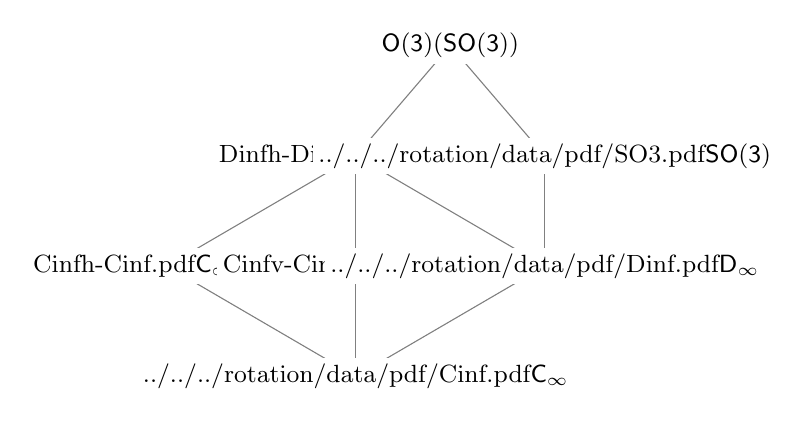
\begin{tikzpicture}[x=1cm, y=1cm, every node/.style={fill=white, font=\small, inner sep=2pt}]
\draw[black!50, line width=0.4pt] (0,0) -- (-2.4,1.4);
\draw[black!50, line width=0.4pt] (0,0) -- (0,1.4);
\draw[black!50, line width=0.4pt] (0,0) -- (2.4,1.4);
\draw[black!50, line width=0.4pt] (-2.4,1.4) -- (0,2.8);
\draw[black!50, line width=0.4pt] (0,1.4) -- (0,2.8);
\draw[black!50, line width=0.4pt] (2.4,1.4) -- (0,2.8);
\draw[black!50, line width=0.4pt] (2.4,1.4) -- (2.4,2.8);
\draw[black!50, line width=0.4pt] (0,2.8) -- (1.2,4.2);
\draw[black!50, line width=0.4pt] (2.4,2.8) -- (1.2,4.2);
\node at (0,0) {\href{../../../rotation/data/pdf/Cinf.pdf}{\textcolor{black}{$\grp{C_{\infty}}$}}};
\node at (-2.4,1.4) {\href{Cinfh-Cinf.pdf}{\textcolor{black}{$\grp{C_{\infty h}}(\grp{C_{\infty}})$}}};
\node at (0,1.4) {\href{Cinfv-Cinf.pdf}{\textcolor{black}{$\grp{C_{\infty v}}(\grp{C_{\infty}})$}}};
\node at (2.4,1.4) {\href{../../../rotation/data/pdf/Dinf.pdf}{\textcolor{black}{$\grp{D_{\infty}}$}}};
\node at (0,2.8) {\href{Dinfh-Dinf.pdf}{\textcolor{black}{$\grp{D_{\infty h}}(\grp{D_{\infty}})$}}};
\node at (2.4,2.8) {\href{../../../rotation/data/pdf/SO3.pdf}{\textcolor{black}{$\grp{SO(3)}$}}};
\node at (1.2,4.2) {\textcolor{black}{$\grp{O(3)}(\grp{SO(3)})$}};
\end{tikzpicture}\end{center}
The table lists the closed subgroups other than $\grp{O(3)}(\grp{SO(3)})$ up to conjugacy in $\grp{O(3)}(\grp{SO(3)})$, one in each row: the continuous subgroups, then those over the members of each family, then those over the exceptional groups. \label{n:index.family.N}A row with $N$ in its symbol stands for every $N$ of its range, and its entries are functions of $N$. \label{n:head.subgroup}\label{n:head.magnetic.type}\label{n:head.order}\label{n:head.conjugates}\label{n:head.normal}A row gives the representative of a class of subgroups (subgrp), its magnetic type (type), its order, the number of subgroups in the class (conjugates) and whether the representative is normal. \label{n:head.normalizer}\label{n:head.centralizer}It also gives its normalizer and its centralizer in $\grp{O(3)}(\grp{SO(3)})$. The record holds the members with $N \le 12$ (\texttt{subgroup\symbol{95}classes}), and the section Closed subgroups of the document of \href{../../../rotation/data/pdf/O3.pdf}{$\grp{O(3)}$} gives other names of some members with $N = 1$.
{\small\begin{longtable}{@{}llrrlll@{}}\toprule
subgrp & type & order & conjugates & normal & normalizer & centralizer\\\midrule\endhead
\bottomrule\endfoot\endlastfoot
\href{../../../rotation/data/pdf/Cinf.pdf}{$\grp{C_{\infty}}$} & I & $\infty$ & $\infty$ & no & \href{Dinfh-Dinf.pdf}{$\grp{D_{\infty h}}(\grp{D_{\infty}})$} & \href{Cinfh-Cinf.pdf}{$\grp{C_{\infty h}}(\grp{C_{\infty}})$}\\*
\href{Cinfh-Cinf.pdf}{$\grp{C_{\infty h}}(\grp{C_{\infty}})$} & III & $\infty$ & $\infty$ & no & \href{Dinfh-Dinf.pdf}{$\grp{D_{\infty h}}(\grp{D_{\infty}})$} & \href{Cinfh-Cinf.pdf}{$\grp{C_{\infty h}}(\grp{C_{\infty}})$}\\
\href{Cinfv-Cinf.pdf}{$\grp{C_{\infty v}}(\grp{C_{\infty}})$} & III & $\infty$ & $\infty$ & no & \href{Dinfh-Dinf.pdf}{$\grp{D_{\infty h}}(\grp{D_{\infty}})$} & \href{C2h-C2.pdf}{$\grp{C_{2h}}(\grp{C_{2}})$}\\
\href{../../../rotation/data/pdf/Dinf.pdf}{$\grp{D_{\infty}}$} & I & $\infty$ & $\infty$ & no & \href{Dinfh-Dinf.pdf}{$\grp{D_{\infty h}}(\grp{D_{\infty}})$} & \href{C2h-C2.pdf}{$\grp{C_{2h}}(\grp{C_{2}})$}\\
\href{Dinfh-Dinf.pdf}{$\grp{D_{\infty h}}(\grp{D_{\infty}})$} & III & $\infty$ & $\infty$ & no & \href{Dinfh-Dinf.pdf}{$\grp{D_{\infty h}}(\grp{D_{\infty}})$} & \href{C2h-C2.pdf}{$\grp{C_{2h}}(\grp{C_{2}})$}\\
\href{../../../rotation/data/pdf/SO3.pdf}{$\grp{SO(3)}$} & I & $\infty$ & 1 & yes & \href{O3-SO3.pdf}{$\grp{O(3)}(\grp{SO(3)})$} & \href{S2-C1.pdf}{$\grp{C_{i}}(\grp{C_{1}})$}\\
\grouprule{0pt}{\lightrulewidth}
\href{../../../rotation/data/pdf/C1.pdf}{$\grp{C_{1}}$} & I & 1 & 1 & yes & \href{O3-SO3.pdf}{$\grp{O(3)}(\grp{SO(3)})$} & \href{O3-SO3.pdf}{$\grp{O(3)}(\grp{SO(3)})$}\\
\href{../../../rotation/data/pdf/C2.pdf}{$\grp{C_{2}}$} & I & 2 & $\infty$ & no & \href{Dinfh-Dinf.pdf}{$\grp{D_{\infty h}}(\grp{D_{\infty}})$} & \href{Dinfh-Dinf.pdf}{$\grp{D_{\infty h}}(\grp{D_{\infty}})$}\\
$\grp{C_{\mathnormal{N}}}$, $N \ge 3$ & I & $N$ & $\infty$ & no & \href{Dinfh-Dinf.pdf}{$\grp{D_{\infty h}}(\grp{D_{\infty}})$} & \href{Cinfh-Cinf.pdf}{$\grp{C_{\infty h}}(\grp{C_{\infty}})$}\\
\grouprule{0pt}{\lightrulewidth}
\href{S2-C1.pdf}{$\grp{C_{i}}(\grp{C_{1}})$} & III & 2 & 1 & yes & \href{O3-SO3.pdf}{$\grp{O(3)}(\grp{SO(3)})$} & \href{O3-SO3.pdf}{$\grp{O(3)}(\grp{SO(3)})$}\\
$\grp{S_{2\mathnormal{N}}}(\grp{C_{\mathnormal{N}}})$, $N \ge 2$ & III & $2N$ & $\infty$ & no & \href{Dinfh-Dinf.pdf}{$\grp{D_{\infty h}}(\grp{D_{\infty}})$} & \href{Cinfh-Cinf.pdf}{$\grp{C_{\infty h}}(\grp{C_{\infty}})$}\\
\grouprule{0pt}{\lightrulewidth}
\href{C2h-C2.pdf}{$\grp{C_{2h}}(\grp{C_{2}})$} & III & 4 & $\infty$ & no & \href{Dinfh-Dinf.pdf}{$\grp{D_{\infty h}}(\grp{D_{\infty}})$} & \href{Dinfh-Dinf.pdf}{$\grp{D_{\infty h}}(\grp{D_{\infty}})$}\\
$\grp{C_{\mathnormal{N}h}}(\grp{C_{\mathnormal{N}}})$, $N \ge 3$ & III & $2N$ & $\infty$ & no & \href{Dinfh-Dinf.pdf}{$\grp{D_{\infty h}}(\grp{D_{\infty}})$} & \href{Cinfh-Cinf.pdf}{$\grp{C_{\infty h}}(\grp{C_{\infty}})$}\\
\grouprule{0pt}{\lightrulewidth}
\href{C1v-C1.pdf}{$\grp{C_{s}}(\grp{C_{1}})$} & III & 2 & $\infty$ & no & \href{Dinfh-Dinf.pdf}{$\grp{D_{\infty h}}(\grp{D_{\infty}})$} & \href{Dinfh-Dinf.pdf}{$\grp{D_{\infty h}}(\grp{D_{\infty}})$}\\
\href{C2v-C2.pdf}{$\grp{C_{2v}}(\grp{C_{2}})$} & III & 4 & $\infty$ & no & \href{D4h-D4.pdf}{$\grp{D_{4h}}(\grp{D_{4}})$} & \href{D2h-D2.pdf}{$\grp{D_{2h}}(\grp{D_{2}})$}\\
$\grp{C_{\mathnormal{N}v}}(\grp{C_{\mathnormal{N}}})$, $N \ge 3$ & III & $2N$ & $\infty$ & no & $\grp{D_{2\mathnormal{N}h}}(\grp{D_{2\mathnormal{N}}})$ & \href{C2h-C2.pdf}{$\grp{C_{2h}}(\grp{C_{2}})$}\\
\grouprule{0pt}{\lightrulewidth}
\href{../../../rotation/data/pdf/D2.pdf}{$\grp{D_{2}}$} & I & 4 & $\infty$ & no & \href{Oh-O.pdf}{$\grp{O_{h}}(\grp{O})$} & \href{D2h-D2.pdf}{$\grp{D_{2h}}(\grp{D_{2}})$}\\
$\grp{D_{\mathnormal{N}}}$, $N \ge 3$ & I & $2N$ & $\infty$ & no & $\grp{D_{2\mathnormal{N}h}}(\grp{D_{2\mathnormal{N}}})$ & \href{C2h-C2.pdf}{$\grp{C_{2h}}(\grp{C_{2}})$}\\
\grouprule{0pt}{\lightrulewidth}
\href{D2h-D2.pdf}{$\grp{D_{2h}}(\grp{D_{2}})$} & III & 8 & $\infty$ & no & \href{Oh-O.pdf}{$\grp{O_{h}}(\grp{O})$} & \href{D2h-D2.pdf}{$\grp{D_{2h}}(\grp{D_{2}})$}\\
$\grp{D_{\mathnormal{N}h}}(\grp{D_{\mathnormal{N}}})$, $N \ge 3$ & III & $4N$ & $\infty$ & no & $\grp{D_{2\mathnormal{N}h}}(\grp{D_{2\mathnormal{N}}})$ & \href{C2h-C2.pdf}{$\grp{C_{2h}}(\grp{C_{2}})$}\\
\grouprule{0pt}{\lightrulewidth}
$\grp{D_{\mathnormal{N}d}}(\grp{D_{\mathnormal{N}}})$, $N \ge 2$ & III & $4N$ & $\infty$ & no & $\grp{D_{2\mathnormal{N}h}}(\grp{D_{2\mathnormal{N}}})$ & \href{C2h-C2.pdf}{$\grp{C_{2h}}(\grp{C_{2}})$}\\
\grouprule{0pt}{\lightrulewidth}
\href{../../../rotation/data/pdf/T.pdf}{$\grp{T}$} & I & 12 & $\infty$ & no & \href{Oh-O.pdf}{$\grp{O_{h}}(\grp{O})$} & \href{S2-C1.pdf}{$\grp{C_{i}}(\grp{C_{1}})$}\\
\href{Th-T.pdf}{$\grp{T_{h}}(\grp{T})$} & III & 24 & $\infty$ & no & \href{Oh-O.pdf}{$\grp{O_{h}}(\grp{O})$} & \href{S2-C1.pdf}{$\grp{C_{i}}(\grp{C_{1}})$}\\
\href{Td-T.pdf}{$\grp{T_{d}}(\grp{T})$} & III & 24 & $\infty$ & no & \href{Oh-O.pdf}{$\grp{O_{h}}(\grp{O})$} & \href{S2-C1.pdf}{$\grp{C_{i}}(\grp{C_{1}})$}\\
\href{../../../rotation/data/pdf/O.pdf}{$\grp{O}$} & I & 24 & $\infty$ & no & \href{Oh-O.pdf}{$\grp{O_{h}}(\grp{O})$} & \href{S2-C1.pdf}{$\grp{C_{i}}(\grp{C_{1}})$}\\
\href{Oh-O.pdf}{$\grp{O_{h}}(\grp{O})$} & III & 48 & $\infty$ & no & \href{Oh-O.pdf}{$\grp{O_{h}}(\grp{O})$} & \href{S2-C1.pdf}{$\grp{C_{i}}(\grp{C_{1}})$}\\
\href{../../../rotation/data/pdf/I.pdf}{$\grp{I}$} & I & 60 & $\infty$ & no & \href{Ih-I.pdf}{$\grp{I_{h}}(\grp{I})$} & \href{S2-C1.pdf}{$\grp{C_{i}}(\grp{C_{1}})$}\\*
\href{Ih-I.pdf}{$\grp{I_{h}}(\grp{I})$} & III & 120 & $\infty$ & no & \href{Ih-I.pdf}{$\grp{I_{h}}(\grp{I})$} & \href{S2-C1.pdf}{$\grp{C_{i}}(\grp{C_{1}})$}\\
\bottomrule\end{longtable}}
\needspace{159pt}
\section{Descent of symmetry}\label{s:subduction}
Conventions: \href{../../CONVENTIONS.pdf}{CONVENTIONS.pdf}, sections \href{../../../rotation/CONVENTIONS.pdf\#conv.12}{12}, \href{../../CONVENTIONS.pdf\#conv.33.1}{33.1} and \href{../../CONVENTIONS.pdf\#conv.37.4}{37.4}.
A row is a family of irreps $\Gamma$ of \href{../../../rotation/data/pdf/O3.pdf}{$\grp{O(3)}$} over $\mathbb{R}$, which are corepresentations of \href{O3-1p.pdf}{$\grp{O(3)1'}$} (\href{../../CONVENTIONS.pdf}{CONVENTIONS.pdf}, section \href{../../CONVENTIONS.pdf\#conv.32.1}{32.1}). A row gives the restriction of $\Gamma$ to $\grp{O(3)}(\grp{SO(3)})$ as a sum of corepresentations (section~\ref{s:families}). A corepresentation of $\grp{O(3)1'}$ splits in $\grp{O(3)}(\grp{SO(3)})$ exactly when its row has more than one term.
{\small\begin{longtable}{@{}ll@{}}\toprule
family & $\restr{\Gamma}{\grp{O(3)}(\grp{SO(3)})}$\\\midrule\endhead
\bottomrule\endfoot\endlastfoot
$\irrJp{J}{+}$ & $\irrJ{J}$\\*
$\irrJp{J}{-}$ & $\irrJ{J}$\\
\bottomrule\end{longtable}}
\needspace{171pt}
\partbox{Angular momentum}
\section{Subduction from \texorpdfstring{$\grp{O(3)1'}$}{O(3)1\unichar{8242}}}\label{s:subduction_o3}
Conventions: \href{../../CONVENTIONS.pdf}{CONVENTIONS.pdf}, sections \href{../../../rotation/CONVENTIONS.pdf\#conv.11}{11}, \href{../../CONVENTIONS.pdf\#conv.33.1}{33.1} and \href{../../CONVENTIONS.pdf\#conv.37.4}{37.4}.
\leavevmode\label{n:index.J}\label{n:index.parity}The irrep $\irrJp{J}{p}$ of $\grp{O(3)1'}$ has angular momentum $J$ and parity $p$ ($\ptag{g}$ for $p = +1$, $\ptag{u}$ for $p = -1$), and time reversal acts on it as on its kets (\href{../../CONVENTIONS.pdf}{CONVENTIONS.pdf}, section \href{../../CONVENTIONS.pdf\#conv.31.1}{31.1}). A corepresentation occurs in its restriction to $\grp{O(3)}(\grp{SO(3)})$ as often as its first irrep occurs in the restriction to $\grp{SO(3)}$ (the section Subduction from $\grp{O(3)}$ of the document of \href{../../../rotation/data/pdf/SO3.pdf}{$\grp{SO(3)}$}). For every $J$,
\begin{equation}\label{e:o3rule}\restr{\irrJp{J}{p}}{\grp{O(3)}(\grp{SO(3)})} = \irrJ{J}\quad\text{for both } p.\end{equation}
The record also holds the restrictions for $J \le 6$ (\texttt{subduction\symbol{95}corepresentations}).
\needspace{171pt}
\partbox{Tensors}
\section{Tensors odd under time reversal}\label{s:time_odd}
Conventions: \href{../../CONVENTIONS.pdf}{CONVENTIONS.pdf}, sections \href{../../../rotation/CONVENTIONS.pdf\#conv.10}{10}, \href{../../../rotation/CONVENTIONS.pdf\#conv.13.2}{13.2} and \href{../../CONVENTIONS.pdf\#conv.35}{35}.
\leavevmode\label{n:head.name.property}A row is a tensor property odd under time reversal that $\grp{O(3)}(\grp{SO(3)})$ allows, by its Jahn symbol (name). \label{n:head.spaces}A row gives the spaces of Cartesian tensors in which its components are read (spaces), by their Jahn symbols in the section Isotypic components of the document of \href{../../../rotation/data/pdf/O3.pdf}{$\grp{O(3)}$}. \label{n:head.irrep}\label{n:head.properties}A row also gives the irrep of $\grp{O(3)}$ at which they are read and the properties in words. The irrep is $\chi$ where the spaces are those of the tensor, and $\chi \irrprod \det$ where they are those of the tensor without its axial factor e (\href{../../CONVENTIONS.pdf}{CONVENTIONS.pdf}, section \href{../../CONVENTIONS.pdf\#conv.35}{35}). The components that $\grp{O(3)}(\grp{SO(3)})$ allows are the copies of that irrep in those spaces.
{\small\setlength{\fillwidth}{\textwidth}\addtolength{\fillwidth}{-6\tabcolsep}\setlength{\colwidth}{0pt}\cellmax{$\jahn{aV\{V^{2}\}}$}\cellmax{$\jahn{aeV^{2}}$}\cellmax{name}\cellmax{$\jahn{aV^{3}}$}\addtolength{\fillwidth}{-\colwidth}\setlength{\colwidth}{0pt}\cellmax{$\jahn{V}$ $\oplus$ $\jahn{e[V^{2}]}$ $\oplus$ $\jahn{V[V^{2}]}$}\cellmax{$\jahn{V}$ $\oplus$ $\jahn{e[V^{2}]}$}\cellmax{spaces}\addtolength{\fillwidth}{-\colwidth}\setlength{\colwidth}{0pt}\cellmax{$\irrJp{0}{-}$}\cellmax{irrep}\addtolength{\fillwidth}{-\colwidth}\setlength{\colwidth}{0pt}\cellmax{the imaginary part of the second-order susceptibility}\cellmax{the imaginary part of optical rectification}\cellmax{the linear magnetoelectric effect}\cellmax{properties}\fillcap\begin{longtable}{@{}lll>{\RaggedRight\arraybackslash}p{\fillwidth}@{}}\toprule
name & spaces & irrep & properties\\\midrule\endhead
\bottomrule\endfoot\endlastfoot
$\jahn{aeV^{2}}$ & $\jahn{V}$ $\oplus$ $\jahn{e[V^{2}]}$ & $\irrJp{0}{-}$ & the linear magnetoelectric effect\\*
$\jahn{aV^{3}}$ & $\jahn{V}$ $\oplus$ $\jahn{e[V^{2}]}$ $\oplus$ $\jahn{V[V^{2}]}$ & $\irrJp{0}{-}$ & the imaginary part of the second-order susceptibility\\*
$\jahn{aV\{V^{2}\}}$ & $\jahn{V}$ $\oplus$ $\jahn{e[V^{2}]}$ & $\irrJp{0}{-}$ & the imaginary part of optical rectification\\
\bottomrule\end{longtable}}
\needspace{214pt}
\section{Multipoles}\label{s:multipoles}
Conventions: \href{../../CONVENTIONS.pdf}{CONVENTIONS.pdf}, sections \href{../../CONVENTIONS.pdf\#conv.35.1}{35.1} and \href{../../CONVENTIONS.pdf\#conv.37.6}{37.6}.
A row is a rank $J$, and the last row gives every rank (\texttt{every\symbol{95}rank}). \label{n:head.multipole.electric}\label{n:head.multipole.electric.toroidal}\label{n:head.multipole.magnetic.toroidal}\label{n:head.multipole.magnetic}A row gives the number of independent multipoles of each kind that $\grp{O(3)}(\grp{SO(3)})$ allows. It is the multiplicity in $\irrJp{J}{p}$ of the trivial irrep of $\grp{O(3)}$ for the electric kinds and of $\chi$ for the magnetic kinds (the section Subduction from $\grp{O(3)}$ of the document of \href{../../../rotation/data/pdf/O3.pdf}{$\grp{O(3)}$}).
{\small\begin{longtable}{@{}rrrrr@{}}\toprule
$J$ & electric & electric toroidal & magnetic toroidal & magnetic\\\midrule\endhead
\bottomrule\endfoot\endlastfoot
0 & 1 & 0 & 0 & 1\\*
1 & 0 & 0 & 0 & 0\\*
2 & 0 & 0 & 0 & 0\\*
3 & 0 & 0 & 0 & 0\\*
4 & 0 & 0 & 0 & 0\\*
\grouprule{0pt}{\lightrulewidth} every & 1 for $J = 0$ & 0 & 0 & 1 for $J = 0$\\
\bottomrule\end{longtable}}
The electric entries at even $J$ and the magnetic entries at odd $J$ count the operators on a spin that $\grp{O(3)}(\grp{SO(3)})$ allows (\href{../../CONVENTIONS.pdf}{CONVENTIONS.pdf}, section \href{../../CONVENTIONS.pdf\#conv.35.1}{35.1}).
\needspace{103pt}
\section{Invariants}\label{s:invariants}
Conventions: \href{../../CONVENTIONS.pdf}{CONVENTIONS.pdf}, sections \href{../../CONVENTIONS.pdf\#conv.31.2}{31.2} and \href{../../CONVENTIONS.pdf\#conv.35.1}{35.1}.
The invariant polynomials of $\grp{O(3)}(\grp{SO(3)})$ in one vector of a kind are those of its image of that kind (section~\ref{s:identification}), in the section Invariant polynomials of the image's document (\texttt{rings}).
\leavevmode\label{n:index.degree.polar}\label{n:index.degree.axial}A row is a degree $a$ in a polar vector even under time reversal. A row gives the number of linearly independent invariants of degree $a$ in it and $b$ in an axial vector odd under time reversal, for $a + b \le 6$.
{\small\begin{longtable}{@{}rrrrrr@{}}\toprule
$a$ & $b = 1$ & $b = 2$ & $b = 3$ & $b = 4$ & $b = 5$\\\midrule\endhead
\bottomrule\endfoot\endlastfoot
1 & 1 & 0 & 1 & 0 & 1\\*
2 & 0 & 2 & 0 & 2 & \\*
3 & 1 & 0 & 2 &  & \\*
4 & 0 & 2 &  &  & \\*
5 & 1 &  &  &  & \\
\bottomrule\end{longtable}}
\leavevmode\label{n:local.component.polar}\label{n:local.component.axial}The record holds their bases for $a + b \le 4$ (\texttt{polynomials}), in the components $u_{x}$, $u_{y}$, $u_{z}$ of the polar vector and $v_{x}$, $v_{y}$, $v_{z}$ of the axial vector. \label{n:head.polynomial}A row is an invariant of the reduced row echelon basis of its degrees (\href{../../CONVENTIONS.pdf}{CONVENTIONS.pdf}, section \href{../../CONVENTIONS.pdf\#conv.35.1}{35.1}). A row gives its degrees $a$ and $b$ and the invariant (polynomial).
{\small\renewcommand{\arraystretch}{1.2}\begin{longtable}{@{}rrl@{}}\toprule
$a$ & $b$ & polynomial\\\midrule\endhead
\bottomrule\endfoot\endlastfoot
1 & 1 & $u_{x}v_{x} + u_{y}v_{y} + u_{z}v_{z}$\\*
1 & 3 & $u_{x}v_{x}^{3} + u_{x}v_{x}v_{y}^{2} + u_{x}v_{x}v_{z}^{2} + u_{y}v_{x}^{2}v_{y} + u_{y}v_{y}^{3} + u_{y}v_{y}v_{z}^{2} + u_{z}v_{x}^{2}v_{z} + u_{z}v_{y}^{2}v_{z} + u_{z}v_{z}^{3}$\\*
2 & 2 & $u_{x}^{2}v_{x}^{2} + 2u_{x}u_{y}v_{x}v_{y} + 2u_{x}u_{z}v_{x}v_{z} + u_{y}^{2}v_{y}^{2} + 2u_{y}u_{z}v_{y}v_{z} + u_{z}^{2}v_{z}^{2}$\\*
2 & 2 & $u_{x}^{2}v_{y}^{2} + u_{x}^{2}v_{z}^{2} - 2u_{x}u_{y}v_{x}v_{y} - 2u_{x}u_{z}v_{x}v_{z} + u_{y}^{2}v_{x}^{2} + u_{y}^{2}v_{z}^{2} - 2u_{y}u_{z}v_{y}v_{z} + u_{z}^{2}v_{x}^{2} + u_{z}^{2}v_{y}^{2}$\\*
3 & 1 & $u_{x}^{3}v_{x} + u_{x}^{2}u_{y}v_{y} + u_{x}^{2}u_{z}v_{z} + u_{x}u_{y}^{2}v_{x} + u_{x}u_{z}^{2}v_{x} + u_{y}^{3}v_{y} + u_{y}^{2}u_{z}v_{z} + u_{y}u_{z}^{2}v_{y} + u_{z}^{3}v_{z}$\\
\bottomrule\end{longtable}}
\end{document}
